%%%%%%%%%%%%%%%%%%%%%%%%%%%%%%%%%%%%%%%%%
% Thin Sectioned Essay
% LaTeX Template
% Version 1.0 (3/8/13)
%
% This template has been downloaded from:
% http://www.LaTeXTemplates.com
%
% Original Author:
% Nicolas Diaz (nsdiaz@uc.cl) with extensive modifications by:
% Vel (vel@latextemplates.com)
%
% License:
% CC BY-NC-SA 3.0 (http://creativecommons.org/licenses/by-nc-sa/3.0/)
%
%%%%%%%%%%%%%%%%%%%%%%%%%%%%%%%%%%%%%%%%%

%----------------------------------------------------------------------------------------
% Packages and other document configurations
%----------------------------------------------------------------------------------------

\documentclass[11pt]{article} % Font size (can be 10pt, 11pt or 12pt) and paper size (remove a4paper for US letter paper)

\usepackage[protrusion=true,expansion=true]{microtype} % Better typography
\usepackage{graphicx} % Required for including pictures
\usepackage{wrapfig} % Allows in-line images

\usepackage{mathpazo} % Use the Palatino font
\usepackage[T1]{fontenc} % Required for accented characters
\linespread{1.275} % Change line spacing here, Palatino benefits from a slight increase by default

\usepackage[margin=1in]{geometry} % Reasonable margin size
\setlength{\parskip}{.3em}
\usepackage{amsmath}
\usepackage[hidelinks]{hyperref}
\usepackage{float}
\usepackage{booktabs}

\makeatletter
\renewcommand\@biblabel[1]{\textbf{#1.}} % Change the square brackets for each bibliography item from '[1]' to '1.'
\renewcommand{\@listI}{\itemsep=0pt} % Reduce the space between items in the itemize and enumerate environments and the bibliography

\renewcommand{\maketitle}{ % Customize the title - do not edit title and author name here, see the TITLE block below
\begin{flushright} % Right align
{\LARGE\@title} % Increase the font size of the title

\vspace{20pt} % Some vertical space between the title and author name

{\large\@author} % Author name
\\\@date % Date

\vspace{20pt} % Some vertical space between the author block and abstract
\end{flushright}
}

%----------------------------------------------------------------------------------------
% Title
%----------------------------------------------------------------------------------------

\title{\textbf{Musical Chairs:}\\ 
\vspace*{0.25em} % Title
How BillBoard rankings influence pop success} % Subtitle

\author{\textsc{Danny Vilela} % Author
\\{New York University}} % Institution

\date{\today} % Date

%----------------------------------------------------------------------------------------

\begin{document}

\maketitle % Print the title section

%----------------------------------------------------------------------------------------
% Essay body
%----------------------------------------------------------------------------------------

\section*{Introduction}

Practically gospel for up-and-coming and star-studded artists alike, the US Billboard is the \textit{de facto} source for determining a particular song's nationwide influence and is paramount to cementing one's self as a musical icon. As a ranking for the nation's top 100 trending songs, the billboard has seen numerous iterations in its attempts to accommodate to ever-changing public outlets --- evolving from including only commercially-available songs to its modern, digital-platform (read: YouTube views, Spotify and Apple Music stream counts, AmazonMP3 and iTunes sales, etc.) inclusive equivalent. \par

In 2013, it was reported that the average iTunes user generates \$12 in music sales. This might not sound like much until you consider that iTunes alone accounted for roughly \$6.9 billion in annual consumer spending on music --- roughly three-fourths of global consumer spending for the 2012/2013 fiscal year. In the years since the music industry has seen a significant array of changes -- particularly in the meteoric rise of streaming services like Spotify and Apple Music. That said, it is evident that the Billboard top 100 accounts for much of this success: a higher profile on the billboard draws attention at the national level and often promotes artists to continue releasing music in hopes of capitalizing on said limelight. Given the possibility of predicting a particular song's success would have widespread utility: artists can better understand their standing within the musical industry, record labels can optimize their artists' position on the top 100, and both can optimize their release schedules to maintain a consistent profit. \par

\section*{Problem}
With the seemingly-unforgiving nature of the public's interests paired with a short-term attention span, a series of poor rankings on the top 100 can quickly fade an artist's relevancy and cause career-crippling effects. Artists who consistently fail to break the top 40 are seldom considered ``successful'' by record companies, investors, and -- most importantly -- the public.

With two sections pertaining to material that is overwhelmingly considered to be within the same field -- English and the humanities -- it is evident that a student would strive to maximize their SAT score by favoring the material tested within the Writing and Critical Reading sections. Our assertion, then, is that the separate Critical Reading and Writing sections on the SAT result in similar scores that do not accurately represent individual reading and writing comprehension skills, and instead serve as a detriment to the standardized exam. This problem is important due to the SAT's omnipresence within numerous dimensions of the socio-educational system and ability to influence social progress: if rich students can afford tutors and improve a single ``major'' skill (English language skills), they are able to more efficiently game the SAT's weaknesses and further contribute to the national achievement gap.

\subsection*{Model Definition}
We can assert that the SAT was unable to \textbf{independently} test writing and critical reading skills if for any Critical Reading score we can closely approximate a Writing score. Therefore, we represent our assertion through a simple linear regression model:
\[ \text{Average writing score} =  \beta_0 + \beta_1 \times \text{Average critical reading score} + \text{random error} \]
Furthermore, we note that since the appropriateness of our assertion's model follows a $\beta_0 = 0$ and $\beta_1 = 1$ -- where there is no significant $\beta_0$ due to our desire to express average writing score as a function of average critical reading score -- we can simplify our model such that average critical reading and average writing scores are consistent with one another:
\[ \text{Average writing score} = \text{Average critical reading score} + \text{random error} \]

\section*{Data Sourcing and Cleaning}
I sourced my data by using NYC's new data initiative, NYC Open Data, which allowed me to access datasets pertaining to different public sectors -- including education -- who have released license-free data to the public. My dataset \href{https://data.cityofnewyork.us/Education/SAT-Results/f9bf-2cp4/}{(\texttt{data.cityofnewyork.us/Education/SAT-Results/f9bf-2cp4/})} reported 2012 SAT scores broken down by the scores pertaining to the critical reading, mathematics, and writing sections. Each observation was a high school, with the reported scores resulting from the mean SAT scores from all 2012 college-bound seniors at that particular high school. The NYC Open Data portal provides a simple ``Export'' to CSV, and so obtaining the data was straightforward.

\subsection*{Variables}
For each observation, the CSV contained six features: school code, school name, number of SAT test takers, critical reading average, math average, and writing average scores (averaged across the $n$ number of SAT test takers at that particular school). Note that this analysis does not weigh a school more favorably for having more test-taking students or having higher average scores per section, since there are factors unrelated to this analysis that may be influencing the number of seniors that take the SAT at any particular school or influence how well they perform (systemic social, financial, and educational accessibility deficiencies being particularly notable).

\subsection*{Regression Validation}
Before approaching a dataset with the mindset of performing a linear regression, it was necessary to validate that the conditions for performing a regression analysis of our data was an appropriate route.
\begin{enumerate}

	\item \textbf{$E(\epsilon_i) = 0\ \forall\ i$}: Although our dataset does sample from numerous different high schools where different socioeconomic influences may be impacting the results returned from each high school, we are interested in the intra-observational relationship between critical reading and writing. In other words, we do not care to compare two schools from completely different socioeconomic backgrounds --- rather, we wish to compare a school's average critical reading score to it's own average writing score.
	
	\item \textbf{$V(\epsilon_i) = 0\ \forall\ i$}: We note that the homoscedasticity within this dataset is referring to the equal playing field for all high school students to achieve a possible 800/800 on any particular section of the SAT. It is \textbf{not} the case that the (critical reading)/(writing) relationship is stronger for some schools than for others.
	
	\item $\epsilon_i$ and $\epsilon_j$ are not correlated with each other for $i \neq j$: This is fundamentally assured due to the randomness of our dataset: it would be impossible to assert that knowing observation 283's expected value will tell us anything about observation 284's (or 285's, 286's, etc.) expected value. The only such case where knowing observation $i$'s expected value would be able to tell us anything about observation $j$'s expected value would be if the same set of seniors that were counted in observation $i$'s expected value were counted towards observation $j$'s expected value. No expected values within our dataset are correlated because it would not be possible for (a senior/group of seniors) enrolled into the school on observation $i$ to also be enrolled into the school on observation $j$. Therefore, there cannot be a correlation between expected values when $i \neq j$.
	
	\item $\epsilon_i \sim N(0,\ \sigma^2)$: Given that our data contains a large number of observations with scores ranging across the score spectrum and an evident clustering of scores towards the mean, we can assume that our data represents a normal distribution.
\end{enumerate}

Because we can show that these assumptions hold, we know that least squares regression is the proper regression to use.

\subsection*{Data Validation}
Upon obtaining the data, I noticed that high schools that were not able to report more than 5 seniors' scores had their entire observation suppressed, leaving the ``s'' character in place of each of their features. This required a line of code within my \textsc{R} script in order to filter out rows where the number of test takers was equal to the string ``s''. Furthermore, the SAT section scores were encoded as character strings, and so my \textsc{R} script also converted each feature into its numerical value.

\section*{Exploratory Data Analysis}
First, let's take a quick look at our data through a scatterplot:

%\begin{figure}[H]
%	\label{Figure 1}
%	\caption{Scatterplot of our high schools' reported scores}
%	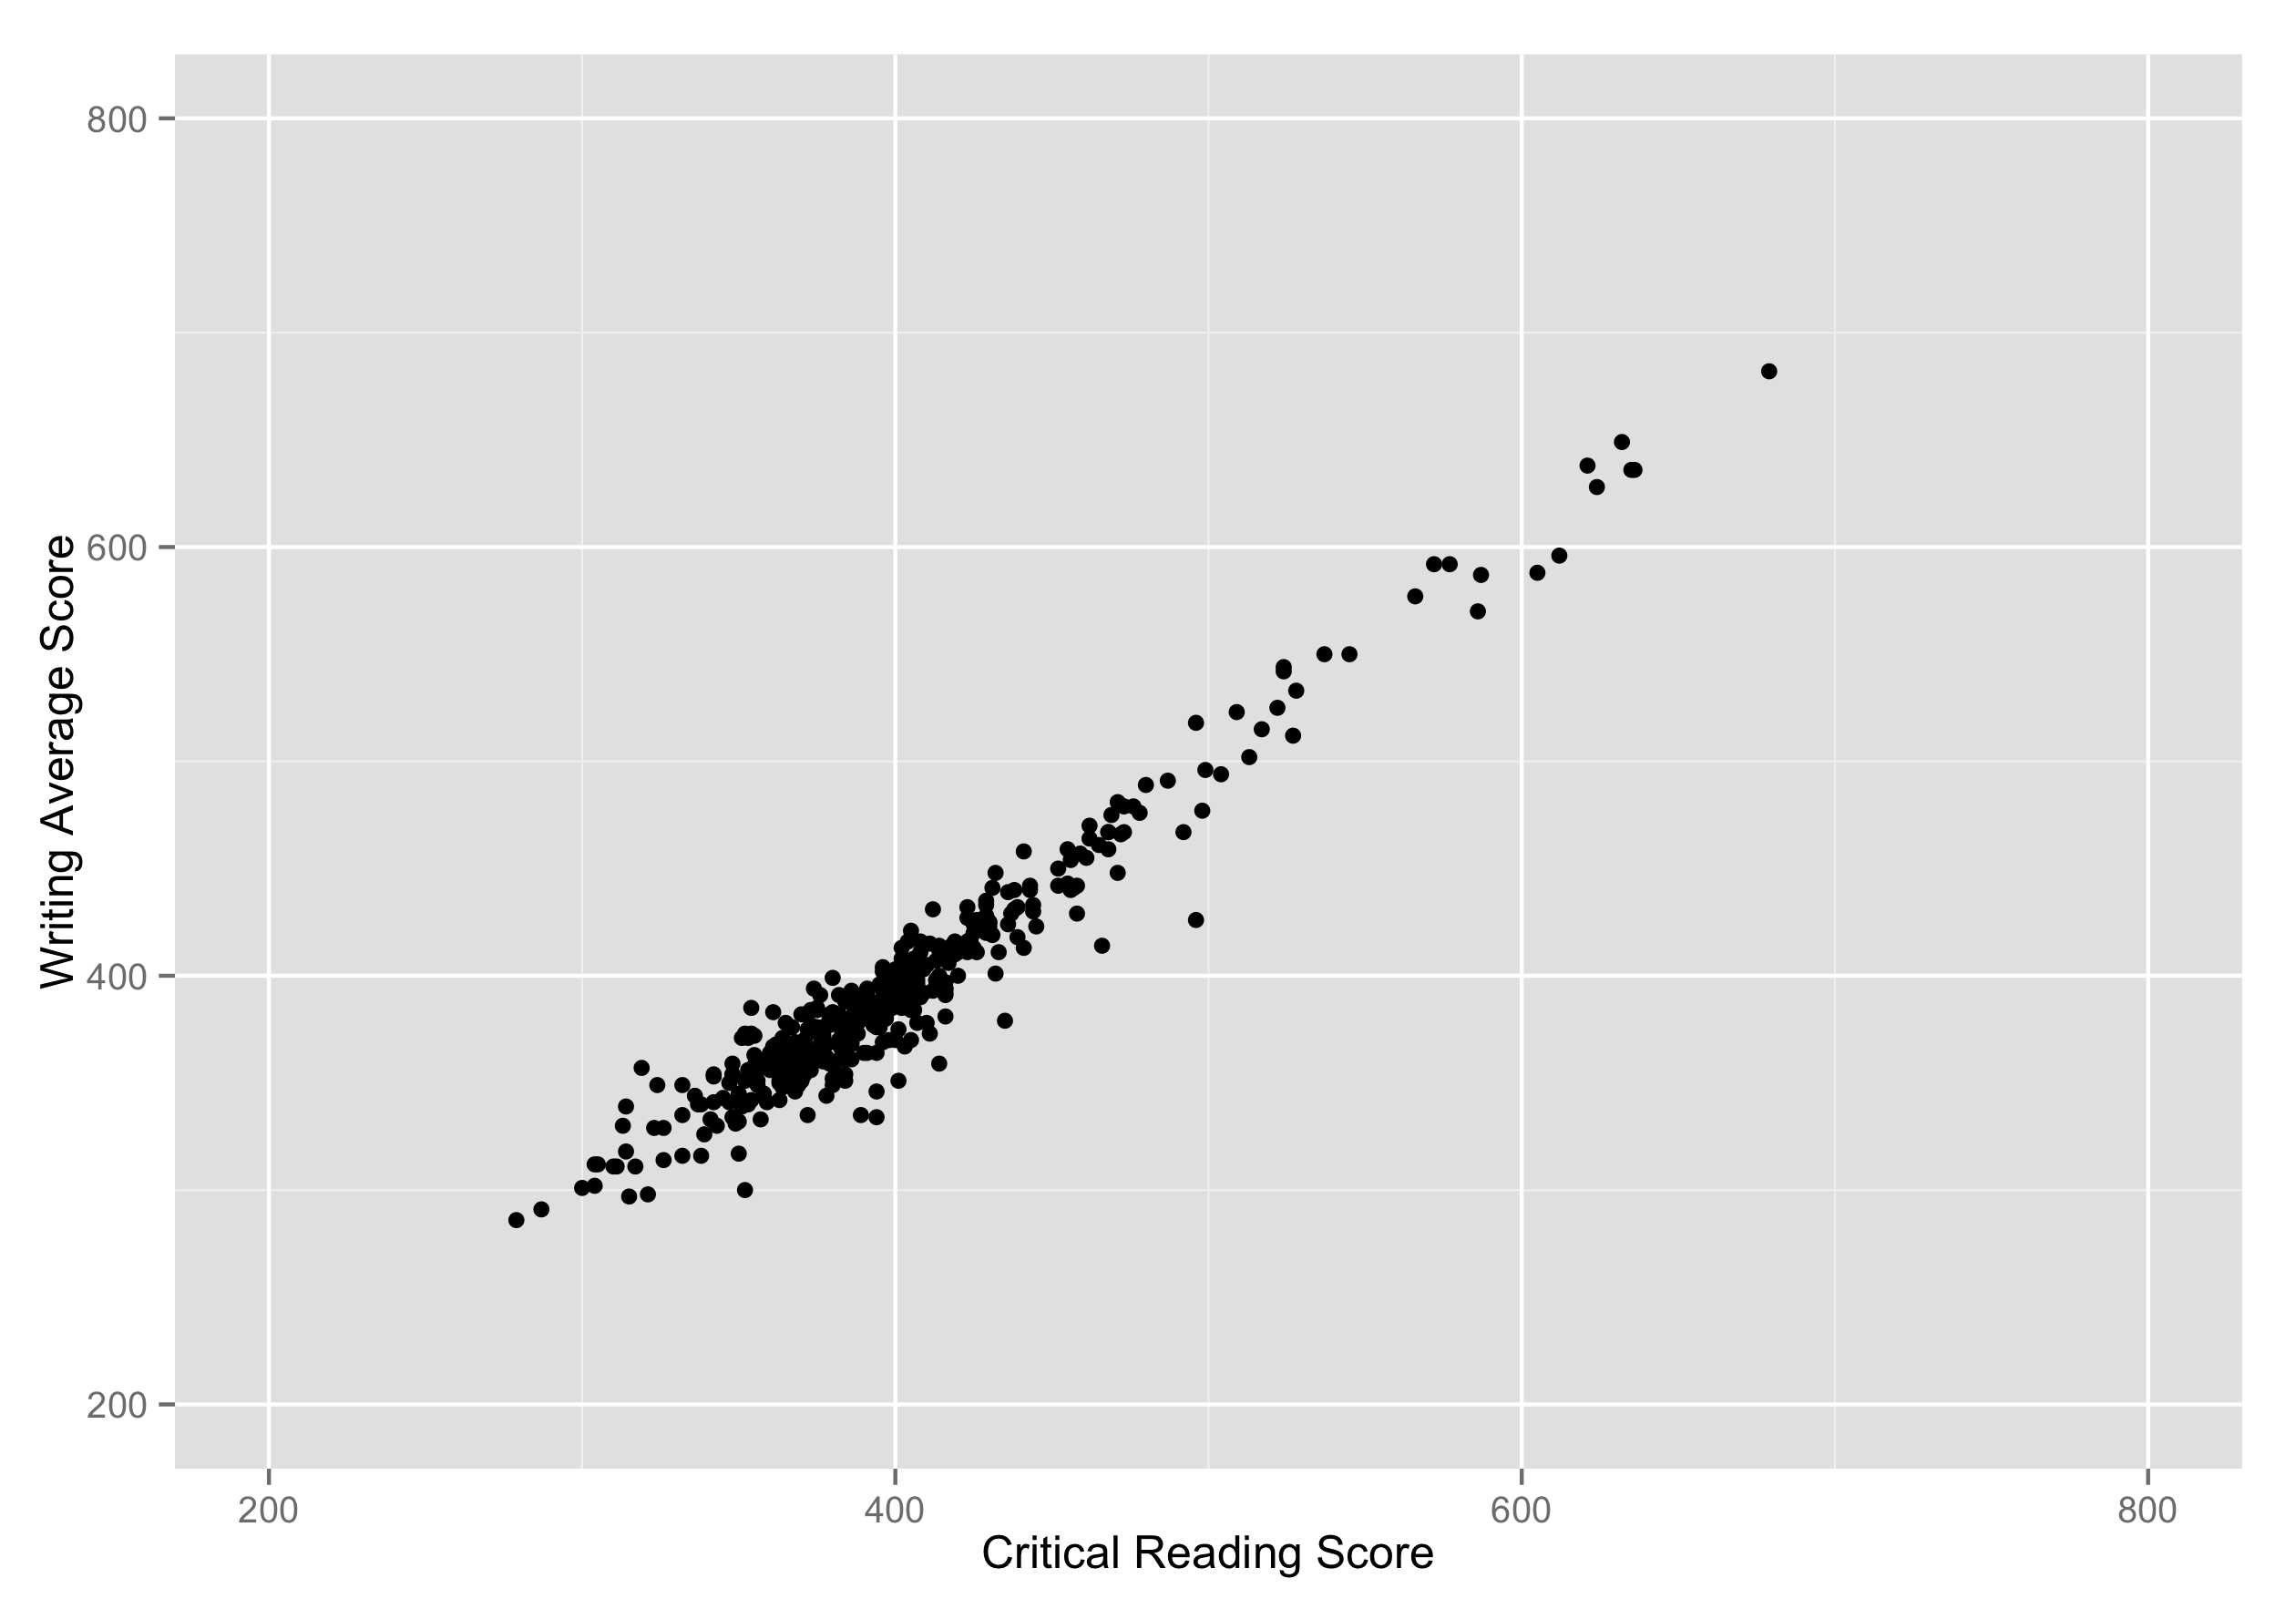
\includegraphics[scale = 0.14]{original_plots/read_v_write_2012}
%	\centering
%\end{figure}

At first glance, there seems to be a very strong linear relationship between average critical reading score and average writing score. We also note that, while most datapoints are centered at the 350 \textasciitilde\ 450 point range (with a thorough range of scores -- ranging from high 200s to low 600s), we have a particularly notable outlier whose averaged scores are at the 680 range while its position is still aligned with our regression line. After utilizing \textsc{R}'s \textit{identify} function, we discover that this school is actually \textit{Stuyvesant High School}, an extremely competitive and well-performing public high school in New York City. \par
Moving on, we perform a least squares regression with average writing score as our dependent (target) variable, and average critical reading score as our independent (predicting) variable:

\begin{verbatim}
------------------------------------------------------------------------------
Residuals:
	  +---------+--------+----------+--------+---------+  
	  |   Min   |   1Q   |  Median  |   3Q   |   Max   |
	  +---------+--------+----------+--------+---------+  
	  | -63.292 | -7.206 |  0.851   | 8.866  | 44.999  |
	  +---------+--------+----------+--------+---------+ 
	
Coefficients:
                  +-----------------+---------+---------+--------------+
                  |  Estimate Std.  |  Error  | t value |   Pr(>|t|)   |
   +--------------+-----------------+---------+---------+--------------+
   |	 (Intercept) |    -7.52321     | 4.93528 |  -1.524 |    0.128 .   |
   +--------------+-----------------+---------+---------+--------------+
   |   CR_Score   |     1.00164     | 0.01219 |  82.166 |  <2e-16 ***  |
   +--------------+-----------------+---------+---------+--------------+
    ---
    Signif. codes:  0 `***' 0.001 `**' 0.01 `*' 0.05 `.' 0.1 ` ' 1
    ---
	
	Residual standard error: 14.19 on 419 degrees of freedom
	Multiple R-squared: 0.9416,	   Adjusted R-squared: 0.9414 
	F-statistic:  6751 on 1 and 419 DF, p-value: < 2.2e-16
------------------------------------------------------------------------------
\end{verbatim}

\noindent We observe that, in accordance with \textsc{R}'s summary, our regression equation becomes:
\[ \texttt{Average writing score} = \texttt{-7.52321} + \texttt{1.00164} \times \texttt{Average critical reading score} \]
We note that our regression is very strong, with an $R^{2}$ of 94.16\%, an adjusted $R^{2}$ of 94.14\%, and a very significant F-statistic of 6751. We also note that the intercept coefficient ($\beta_0$) is not relevant to our findings, because by default the SAT is structured such that the lowest score you can obtain on any section is 200. Our slope coefficient ($\beta_1$), however, signifies that a one point increase in mean critical reading score is associated with an estimated expected 1.00164 point increase in our mean writing score.

\subsection*{Testing the Null Hypothesis}
Our t-statistic given in the output for our linear regression's output in \texttt{CR\_Score} examines the null hypothesis of $\beta_1 = 0$, which is strongly rejected. Despite the strong rejection of the null hypothesis, we can clearly observe a relationship between our critical reading scores and writing scores. That said, if we refer back to our original assertion, it states that our model would support a $\beta_1 = 1$. Furthermore, our original assertion states that $\beta_0 = 0$ because of our interest in whether average critical reading scores can directly -- and independently -- predict average writing scores. \par
Furthermore, the t-statistic for our average writing score can be calculated manually (assuming our model corresponds to a $\beta_1 = 1$):
\[ t = \frac{1.00164 - 1}{14.19} \approx 0.0001 \]

Factoring in our reported standard error of the estimate of 3.76 allows us to observe that this model shows signs of extreme relevance, providing a prediction of writing score to within $\pm$ 7.52 points approximately 95\% of the time. 

\section*{Confidence and Prediction Intervals}
We can observe our 95\% confidence and prediction intervals on a scatterplot:
%\begin{figure}[H]
%	\label{Figure 2}
%	\caption{95\% confidence and prediction intervals for our regression model, plotted.}
%	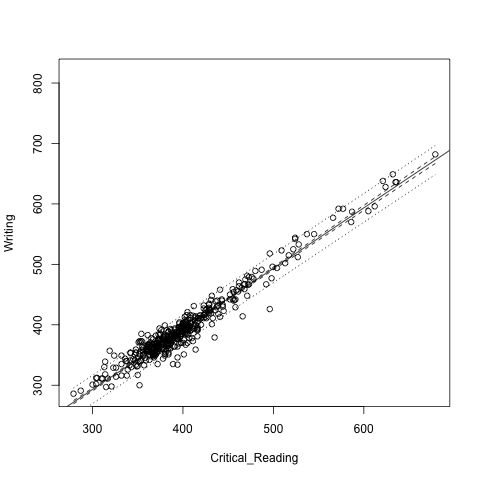
\includegraphics[scale = 0.53]{original_plots/fitted_line_plot_2012}
%	\centering
%\end{figure}
We notice that our confidence interval (short, dashed lines) is nearly overlapping our regression line while our prediction interval (pointwise lines) has a much wider margin in relation to our regression line and confidence interval, simply due to the prediction interval's incorporation of our writing score's variability (whereas our confidence interval does not).


\section*{Interpreting Unusual Data}
Figure 2 also highlights a number of points within the dataset that fall far outside of the 95\% prediction interval -- one of the most notable being ``GED PLUS s CITYWIDE'', a GED program whose college-bound students averaged a 496 on the critical reading section and a 426 on the writing section. A potential explanation for this deviation from the regression line -- aside from the educational impact of GED students often having to balance work and GED fulfillment classes -- is that only 8 seniors had their grades averaged, and so using the mean of 8 data points may be a misleading measurement of central tendency due to the sparse data. We can further observe any unusual data points through diagnostic plots, which can tell us more about whether our assumptions of least squares regressions hold for this particular data. The following plots represent our data's residuals and our residual values versus fitted values:

%\begin{figure}[H]
%	\label{Figure 3}
%	\caption{A normality plot with a significant amount of low outliers, potentially indicating right skewness within the dataset}
%	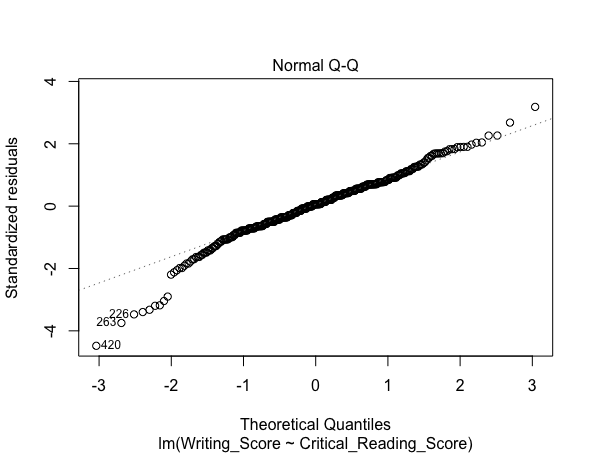
\includegraphics[scale = 0.65]{original_plots/normal_qq}
%	\centering
%\end{figure}

\newpage
%\begin{figure}[H]
%	\label{Figure 4}
%	\caption{A residuals vs fitted plot where we can see a rough horizontal band around the 0 line, if not a partial positive skew}
%	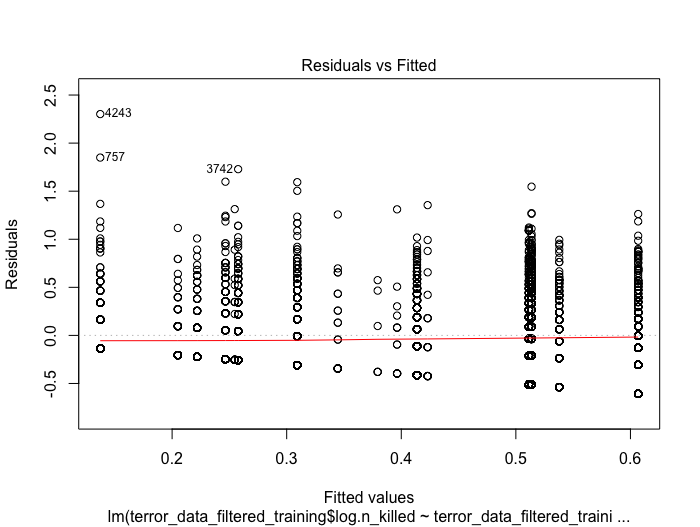
\includegraphics[scale = 0.52]{original_plots/residuals_vs_fitted}
%	\centering
%\end{figure}

Through our plots, we note that observations 226, 263, and 420 are particularly unusual. Whereas observations 226 (``Bronx Aerospace High School'') and 263 (``Juan Morel Campos Secondary School'') did not show outstanding residual values -- with Bronx Aerospace scoring 388 and 382 while Juan Morel scoring 365 and 369 on critical reading and writing scores, respectively -- observation 420 (``Queens Satellite High School for Opportunity'') reported an average score of 403 on critical reading and 367 on writing. \par
One can speculate -- given the lack of documented history -- regarding ``Queens Satellite High School for Opportunity'' that the exceptional residual can be traced back to the dataset's method of aggregating scores: the mean. By its design, the mean of any dataset can provide a useful statistic for measuring central tendency, however, one main disadvantage is that the mean is particularly susceptible to the influence of outliers. Given that the school just barely met the criteria for not suppressing their score -- with 6 high school seniors representing the high school -- if would be possible for one or more of the seniors to perform exceptionally poorly on the writing section while performing at the average, expected level for the critical reading section (given the SATs history with complaints regarding its writing section's scoring criteria, this seems more likely than the case where the seniors did poorly on the critical reading section). These below-expected scores can dramatically shift our mean, and as such will influence our regression model by contributing a notable lower outlier to our data set.

\section*{Outlier Omission}
\subsection*{Omitting $o_1$}
In order to understand the effect of including the outlier ``Queens Satellite High School for Opportunity'' in our regression, we will examine our regression model after removing the outlier. In order to omit this particular school, I modified my \textsc{R} script such that our dataframe \texttt{df} was assigned the rows of \texttt{df} where the \texttt{SCHOOL.NAME} field was not equal to ``QUEENS SATELLITE HIGH SCHOOL FOR OPPORTUNITY''. \par
The scatterplot, without our outlier, is as follows:
%\begin{figure}[H]
%	\label{Figure 5}
%	\caption{Scatterplot of our high schools' reported scores, one outlier removed ($o_1$)}
%	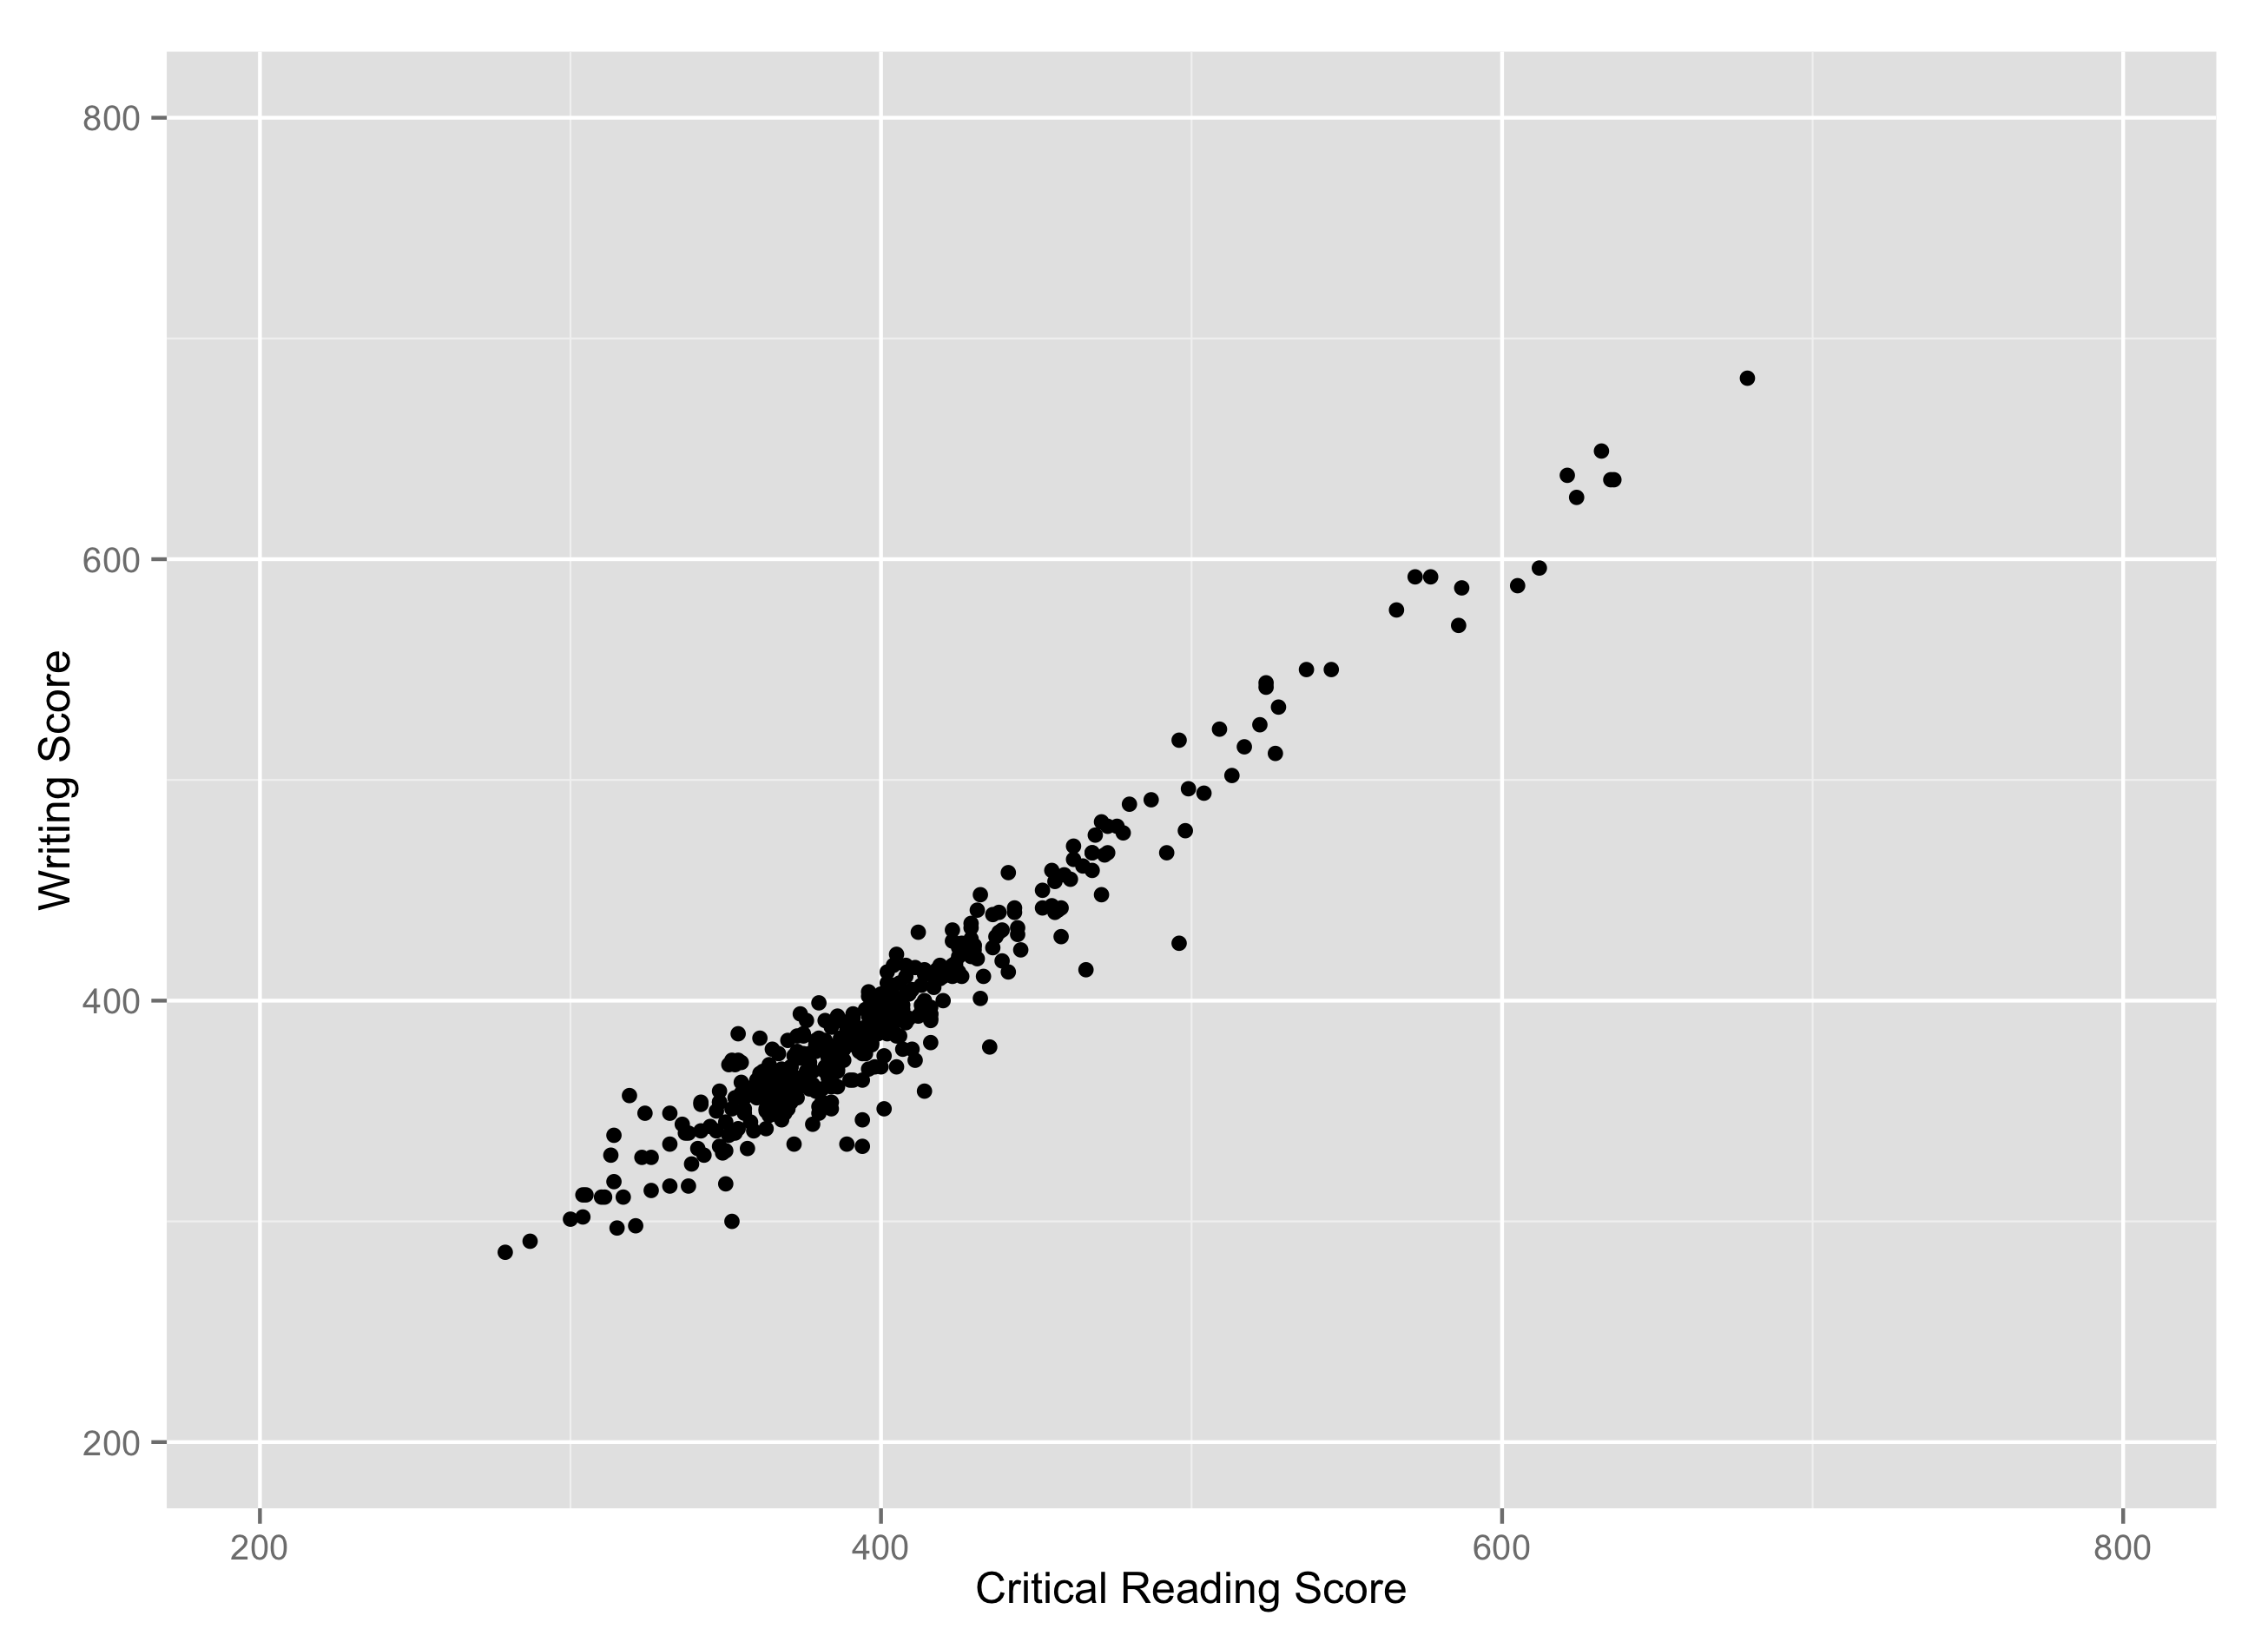
\includegraphics[scale = 0.13]{o_1_removed_plots/read_v_write_2012_altered}
%	\centering
%\end{figure}

We still note a few unusual points (including ``GED PLUS s CITYWIDE'') as marginally unusual. Looking to \textsc{R}'s regression output:

\begin{verbatim}
------------------------------------------------------------------------------
Residuals:
	  +---------+--------+----------+--------+---------+  
	  |   Min   |   1Q   |  Median  |   3Q   |   Max   |
	  +---------+--------+----------+--------+---------+  
	  | -63.366 | -7.240 |  0.784   | 8.797  | 44.934  |
	  +---------+--------+----------+--------+---------+ 
	
\end{verbatim}

\newpage
\begin{verbatim}
Coefficients:
                  +-----------------+---------+---------+--------------+
                  |  Estimate Std.  |  Error  | t value |   Pr(>|t|)   |
   +--------------+-----------------+---------+---------+--------------+
   |	 (Intercept) |    -7.47240     | 4.91626 |  -1.52  |    0.129 .   |
   +--------------+-----------------+---------+---------+--------------+
   |   CR_Score   |     1.00169     | 0.01214 |  82.49  |  <2e-16 ***  |
   +--------------+-----------------+---------+---------+--------------+
    ---
    Signif. codes:  0 `***' 0.001 `**' 0.01 `*' 0.05 `.' 0.1 ` ' 1
    ---
	
	Residual standard error: 14.14 on 418 degrees of freedom
	Multiple R-squared: 0.9421,	    Adjusted R-squared: 0.942
	F-statistic:  6804 on 1 and 418 DF,  p-value: < 2.2e-16
------------------------------------------------------------------------------
\end{verbatim}
\[ \texttt{Average writing score} = \texttt{-7.4724} + \texttt{1.00169} \times \texttt{Average critical reading score} \]
While the regression relationship is still very strong, our $\beta_1$ coefficient is almost insignificantly farther away from our hypothesized value of $\beta_1 = 1$. Looking to our prediction/confidence and diagnostic plots, we note that our confidence interval is still missing a few egregious data points, especially the observation ``GED PLUS s CITYWIDE'':

%\begin{figure}[H]
%	\label{Figure 6}
%	\caption{Confidence and prediction interval plot for our regression model with a removed lower outlier ($o_1$)}
%	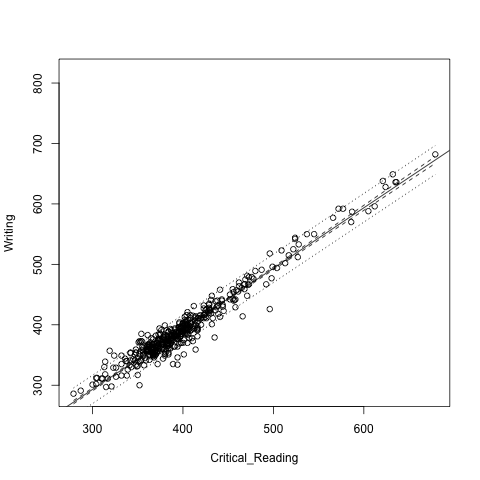
\includegraphics[scale= 0.53]{o_1_removed_plots/fitted_line_plot_2012_altered}
%	\centering
%\end{figure}

%\begin{figure}[H]
%	\label{Figure 7}
%	\caption{Normality plot with a removed lower outlier ($o_1$)}
%	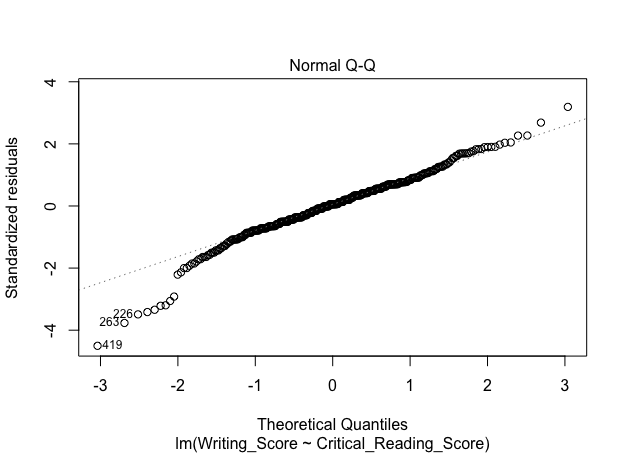
\includegraphics[scale = 0.53]{o_1_removed_plots/qq_2012_altered}
%	\centering
%\end{figure}

%\begin{figure}[H]
%	\label{Figure 8}
%	\caption{Residuals vs fitted plot with a removed lower outlier ($o_1$)}
%	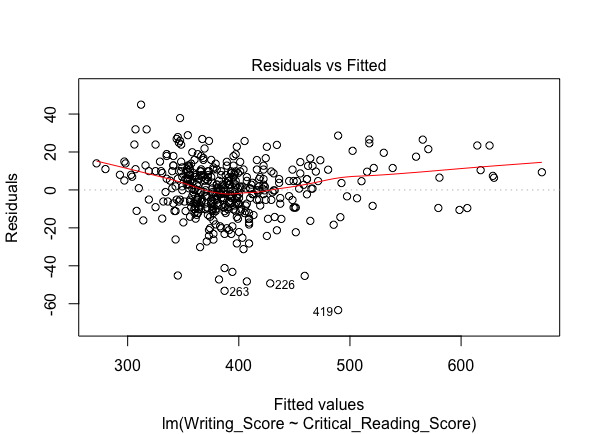
\includegraphics[scale = 0.60]{o_1_removed_plots/residuals_vs_fitted_altered}
%	\centering
%\end{figure}

\subsection*{Omitting $o_2$}
Unfortunately, we can still observe outliers -- particularly within our prediction and confidence interval plot. What if were to re-add our previous outlier and instead remove the ``GED PLUS s CITYWIDE'' outlier from our regression? In order to omit this particular school, I modified my \textsc{R} script such that our dataframe \texttt{df} was assigned the rows of \texttt{df} where the \texttt{SCHOOL.NAME} field was not equal to ``GED PLUS s CITYWIDE''. \par
Here's the scatterplot:

%\begin{figure}[H]
%	\label{Figure 9}
%	\caption{Scatterplot of our reported scores, second outlier ($o_2$) removed, first outlier ($o_1$) intact}
%	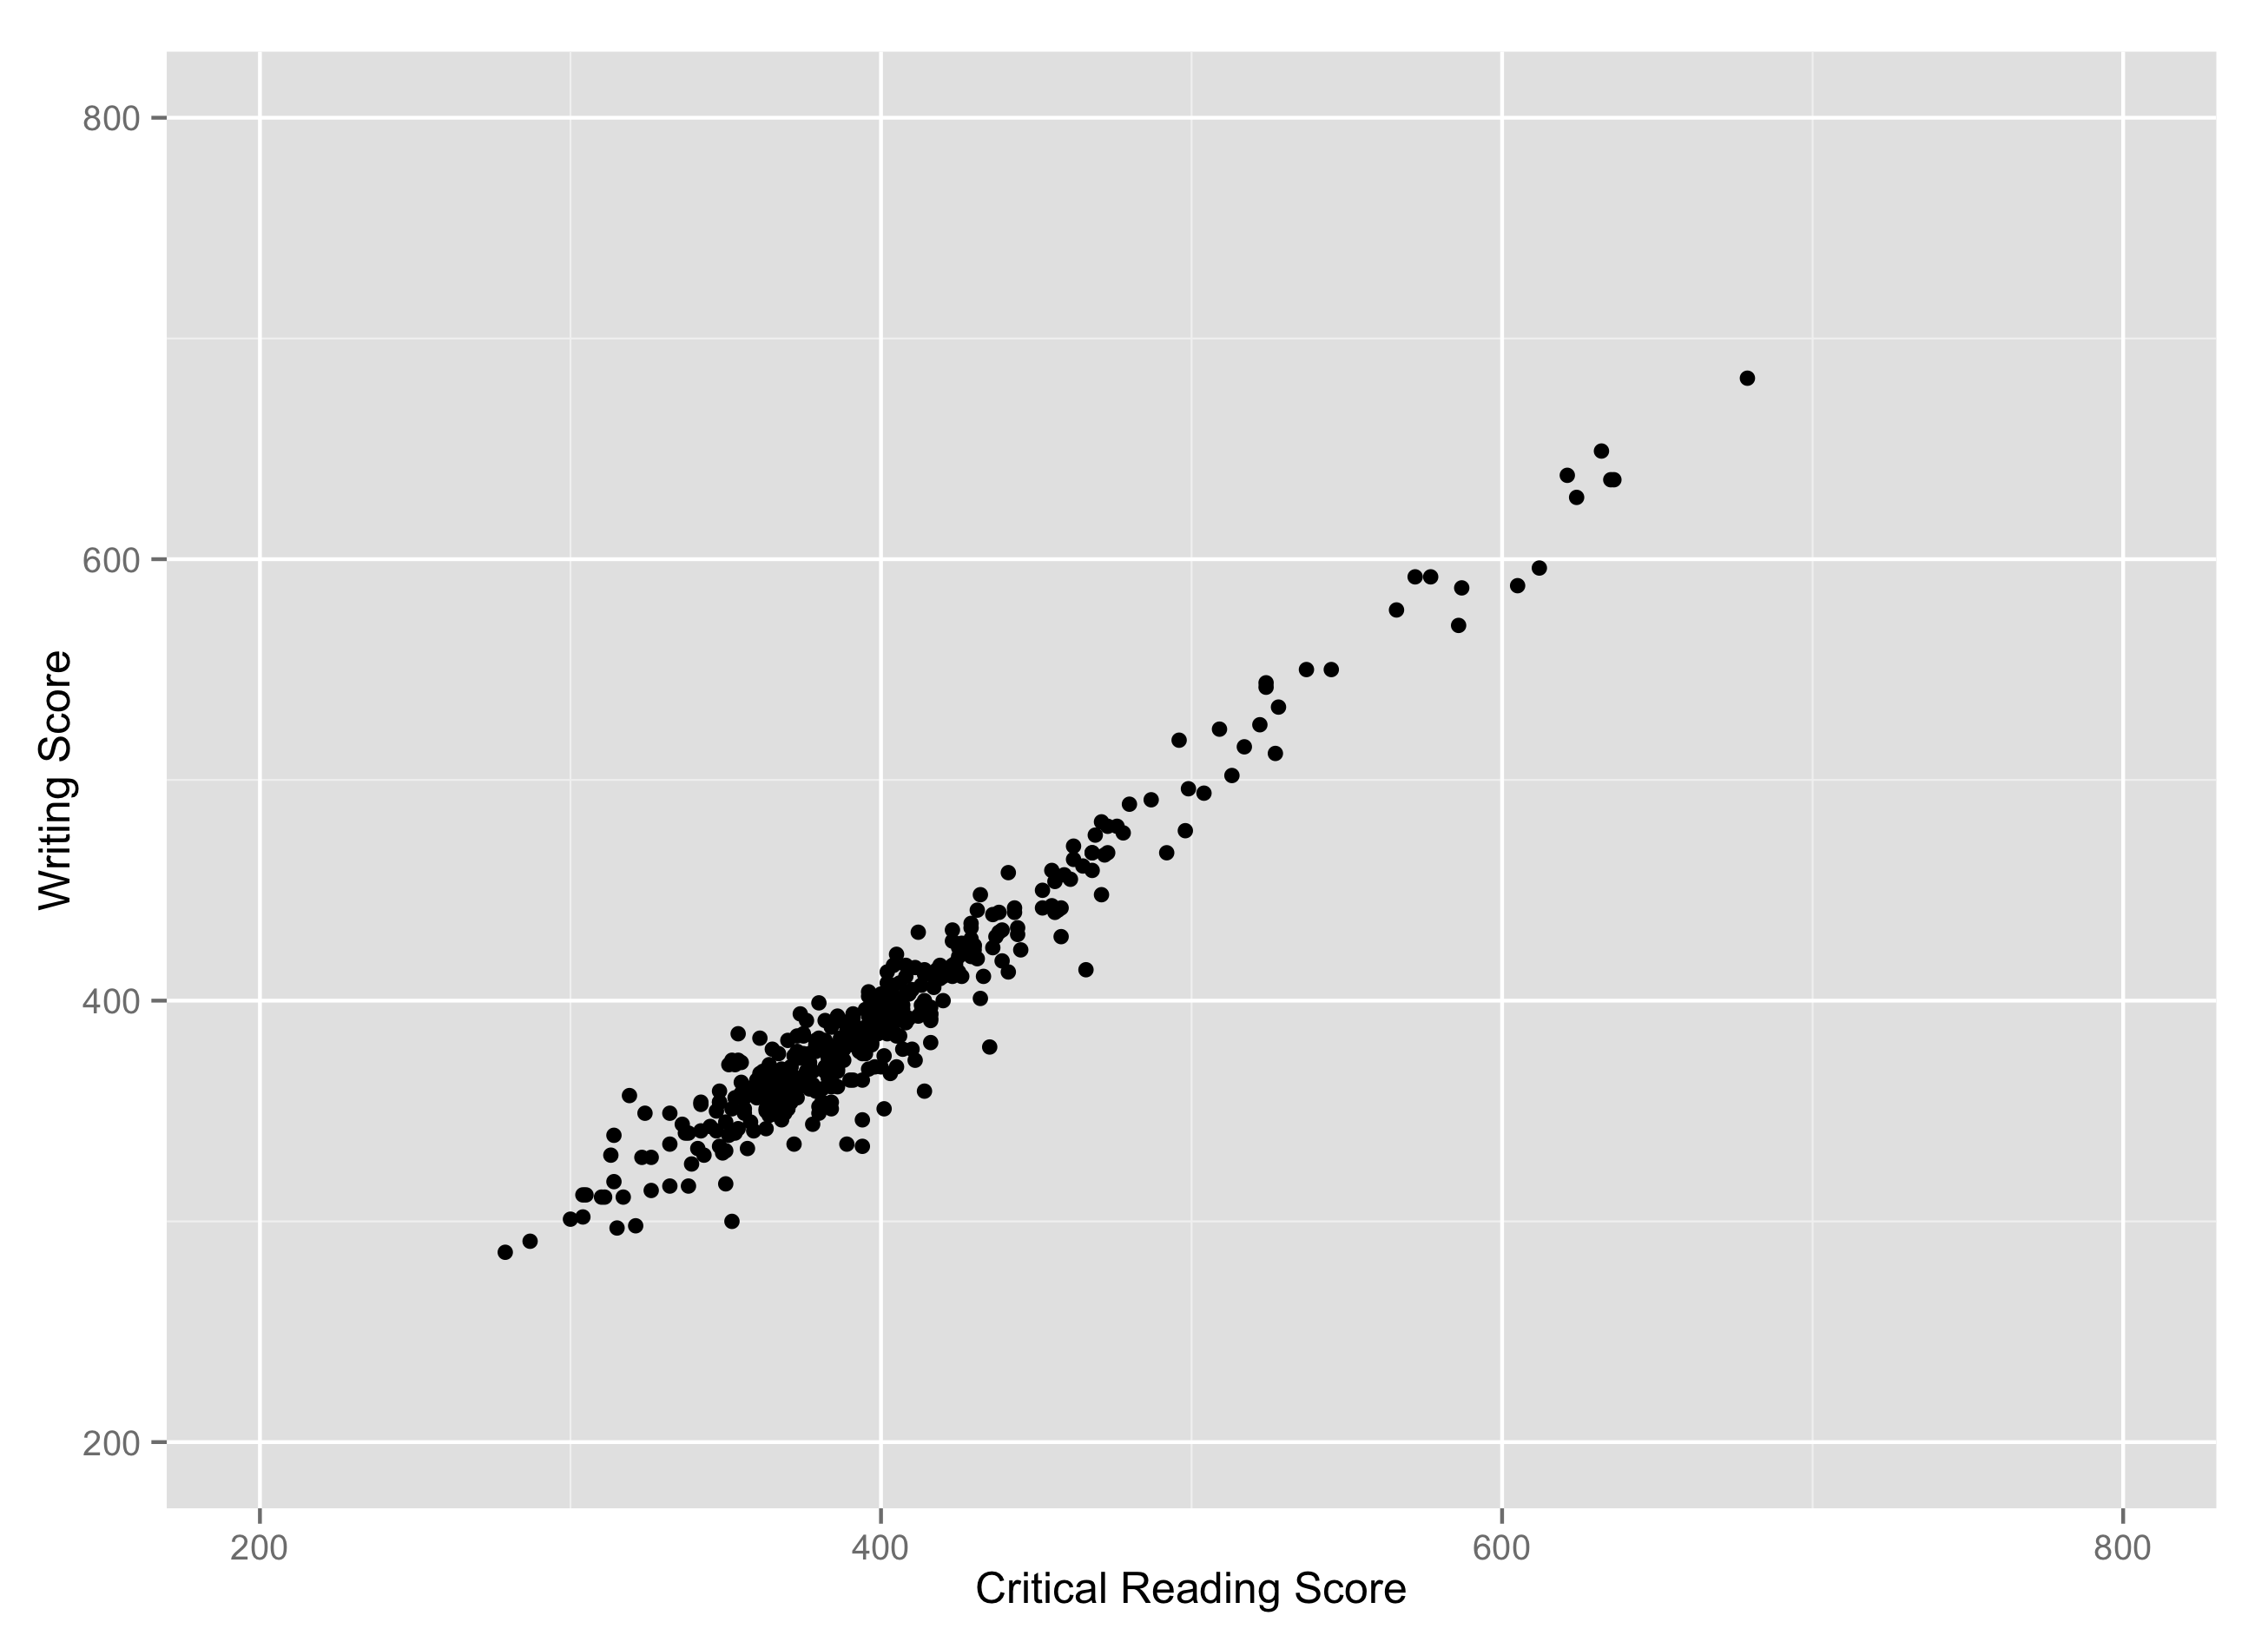
\includegraphics[scale=0.125]{o_2_removed_plots/read_v_write_2012_altered_2}
%	\centering
%\end{figure}

And summary statistics from our regression:

\begin{verbatim}
------------------------------------------------------------------------------
Residuals:
	  +---------+--------+----------+--------+---------+  
	  |   Min   |   1Q   |  Median  |   3Q   |   Max   |
	  +---------+--------+----------+--------+---------+  
	  | -53.245 | -7.414 |  0.672   | 8.704  | 45.214  |
	  +---------+--------+----------+--------+---------+ 
	
Coefficients:
                  +-----------------+---------+---------+--------------+
                  |  Estimate Std.  |  Error  | t value |   Pr(>|t|)   |
   +--------------+-----------------+---------+---------+--------------+
   |	 (Intercept) |    -9.16912     | 4.83471 |  -1.897 |    0.0586 .   |
   +--------------+-----------------+---------+---------+--------------+
   |   CR_Score   |     1.00613     | 0.01195 |  84.200 |  <2e-16 ***  |
   +--------------+-----------------+---------+---------+--------------+
    ---
    Signif. codes:  0 `***' 0.001 `**' 0.01 `*' 0.05 `.' 0.1 ` ' 1
    ---
	
    Residual standard error: 13.86 on 418 degrees of freedom
    Multiple R-squared: 0.9443,    Adjusted R-squared: 0.9442 
    F-statistic:  7090 on 1 and 418 DF,  p-value: < 2.2e-16
------------------------------------------------------------------------------
\end{verbatim}
\[ \text{Average writing score} = -9.16912 + 1.00613 \times \text{Average critical reading score}\]

We notice that removing ``GED PLUS s CITYWIDE'' had a more dramatic effect than removing ``Queens Satellite High School for Opportunity'', but our omission actually brings our $\beta_1$ away from its ideal value of $1$ moreso than omitting ``Queens Satellite High School for Opportunity'' did. Thus, we note that the strength of the relationship between average writing score and average critical reading score has weakened. Let's look at the 95\% confidence/prediction interval plots and the diagnostic plots:

%\begin{figure}[H]
%	\label{Figure 10}
%	\caption{Confidence and prediction interval plot for our regression model with a removed lower outlier ($o_2$); previous outlier ($o_1$) intact}
%	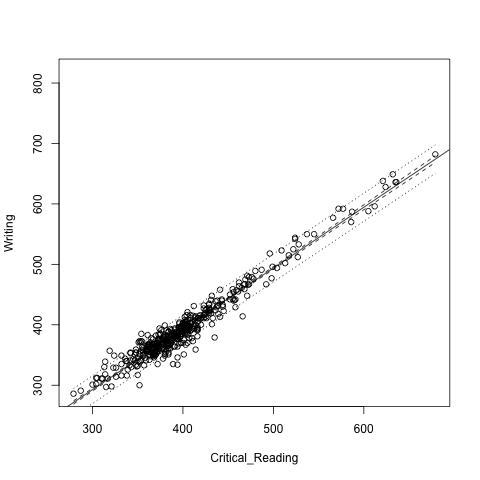
\includegraphics[scale= 0.53]{o_2_removed_plots/fitted_line_plot_2012_altered_2}
%	\centering
%\end{figure}

%\begin{figure}[H]
%	\label{Figure 11}
%	\caption{Normality plot with a removed lower outlier ($o_2$); previous outlier ($o_1$) intact}
%	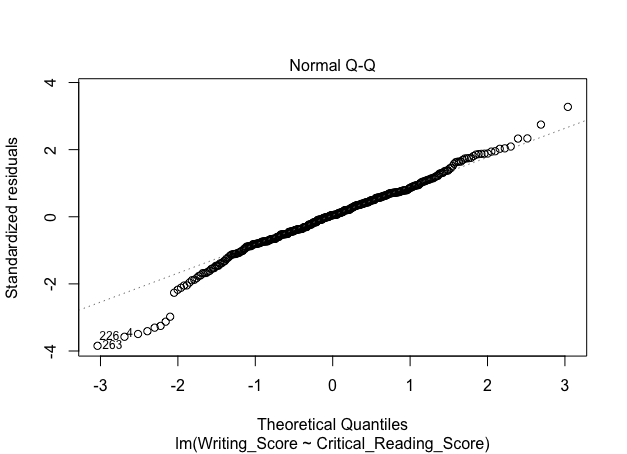
\includegraphics[scale = 0.53]{o_2_removed_plots/qq_2012_altered_2}
%	\centering
%\end{figure}

%\begin{figure}[H]
%	\label{Figure 12}
%	\caption{Residuals vs fitted plot with a removed lower outlier ($o_2$); previous outlier ($o_1$) intact}
%	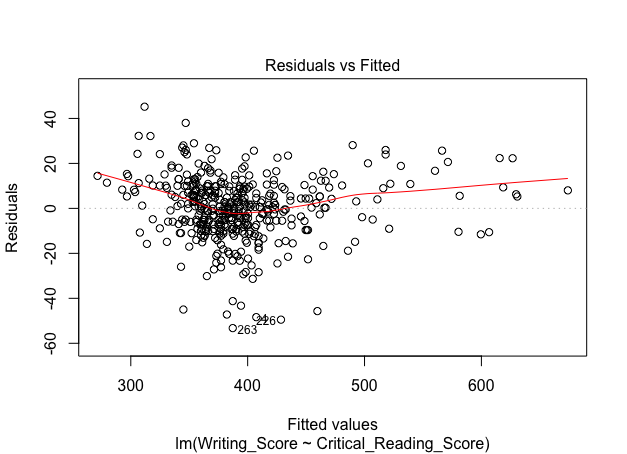
\includegraphics[scale = 0.60]{o_2_removed_plots/residuals_vs_fitted_altered_2}
%	\centering
%\end{figure}

Given $o_2$'s more drastic influence upon our dataset, we arrive at the question: what happens to our linear regression if we remove both notable outliers?

\subsection*{Omitting $o_1$ and $o_2$}
Lastly, we're curious in what will happen to our regression line when we omit both outliers. In order to omit both observations, I modified my \textsc{R} script such that both previous one-line modifications were applied onto my dataframe \texttt{df}. \par
Ideally, the omission of both outliers would provide a $\beta_1$ coefficient that is closer to our ideal value of $1$, and so we first look at our general scatterplot:

%\begin{figure}[H]
%	\label{Figure 13}
%	\caption{Scatterplot of our reported scores both outliers ($o_1$, $o_2$) removed}
%	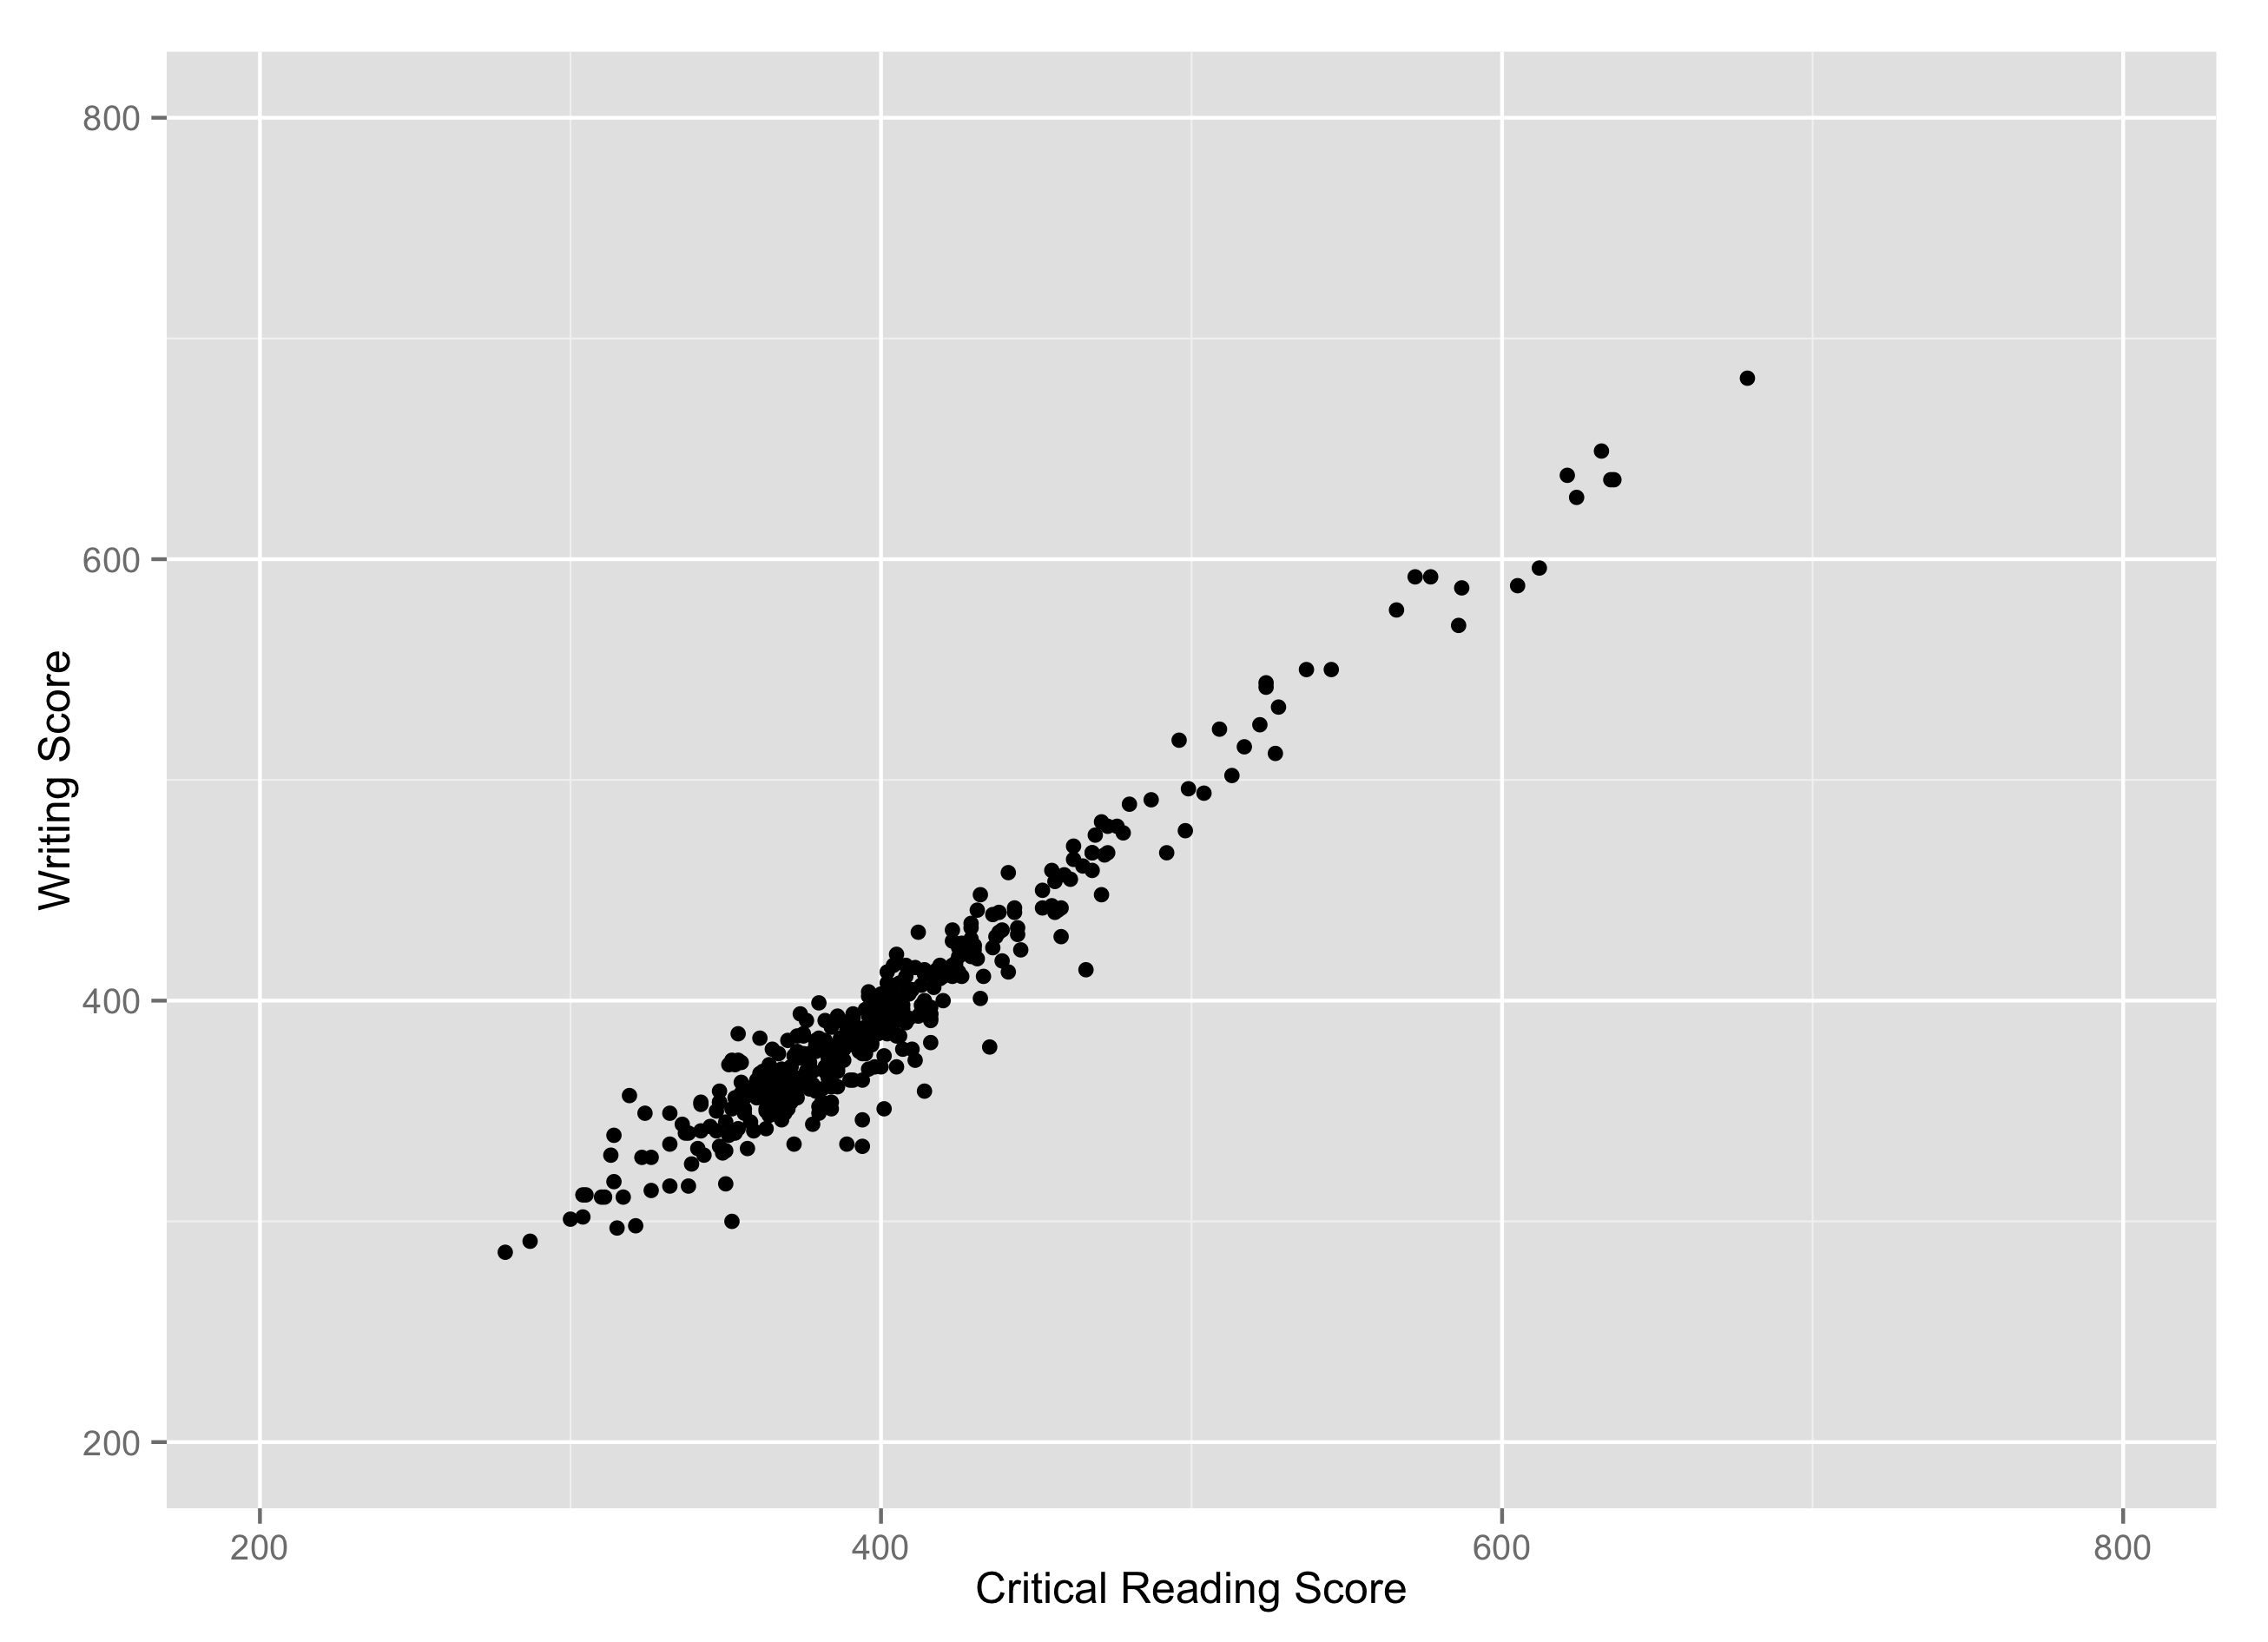
\includegraphics[scale=0.11]{both_removed_plots/read_v_write_2012_altered_final}
%	\centering
%\end{figure}

Followed by \textsc{R}'s summary statistics:

\begin{verbatim}
------------------------------------------------------------------------------
Residuals:
	  +---------+--------+----------+--------+---------+  
	  |   Min   |   1Q   |  Median  |   3Q   |   Max   |
	  +---------+--------+----------+--------+---------+  
	  | -53.315 | -7.417 |  0.611   | 8.639  | 45.149  |
	  +---------+--------+----------+--------+---------+ 
\end{verbatim}
\newpage
\begin{verbatim}
Coefficients:
                  +-----------------+---------+---------+--------------+
                  |  Estimate Std.  |  Error  | t value |   Pr(>|t|)   |
   +--------------+-----------------+---------+---------+--------------+
   |	 (Intercept) |    -9.1200     |  4.8146 |  -1.894 |    0.0589 .   |
   +--------------+-----------------+---------+---------+--------------+
   |   CR_Score   |     1.0062     |  0.0119 |  84.558 |  <2e-16 ***  |
   +--------------+-----------------+---------+---------+--------------+
    ---
    Signif. codes:  0 `***' 0.001 `**' 0.01 `*' 0.05 `.' 0.1 ` ' 1
    ---
	
    Residual standard error: 13.81 on 417 degrees of freedom
    Multiple R-squared: 0.9449,    Adjusted R-squared: 0.9448 
    F-statistic:  7150 on 1 and 417 DF,  p-value: < 2.2e-16
------------------------------------------------------------------------------
\end{verbatim}
The summary of our linear regression results in the following regression equation:
\[ \text{Average writing score} = -9.1200 + 1.0062 \times \text{Average critical reading score}\]

We note a strong $R^{2}$ of 94.49\%, adjusted $R^{2}$ of 94.48\%, and very significant F-statistic of 7150. As usual, our $\beta_0$ does not hold much significance to our regression model due to the minimum score on each section being a 200. Our slope coefficient ($\beta_1$), however, implies that a one point increase in mean critical reading score is associated with an estimated expected 1.0062 point increase in our mean writing score.\par
Lastly, let's take a look at our prediction/confidence interval and diagnostic plots:

%\begin{figure}[H]
%	\label{Figure 14}
%	\caption{Fitted line plot of our reported scores where both outliers ($o_1$, $o_2$) have been removed}
%	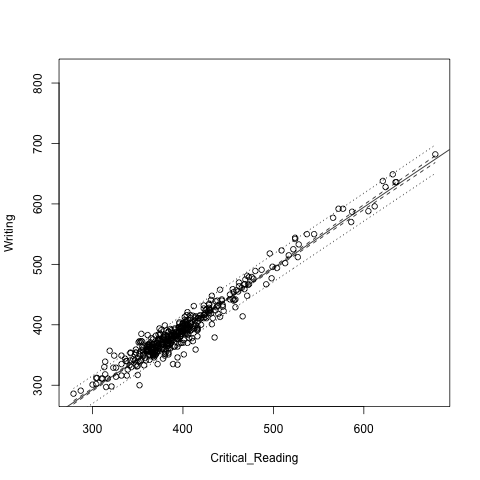
\includegraphics[scale=0.5]{both_removed_plots/fitted_line_plot_2012_altered_final}
%	\centering
%\end{figure}
%
%\begin{figure}[H]
%	\label{Figure 15}
%	\caption{Scatterplot of our reported scores both outliers ($o_1$, $o_2$) removed}
%	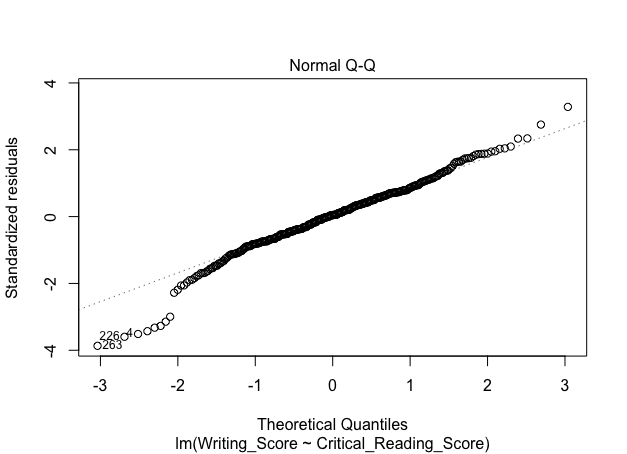
\includegraphics[scale=0.5]{both_removed_plots/qq_normal_altered_final}
%	\centering
%\end{figure}

%\begin{figure}[H]
%	\label{Figure 16}
%	\caption{Scatterplot of our residuals vs our fitted line plot where both outliers ($o_1$, $o_2$) are removed}
%	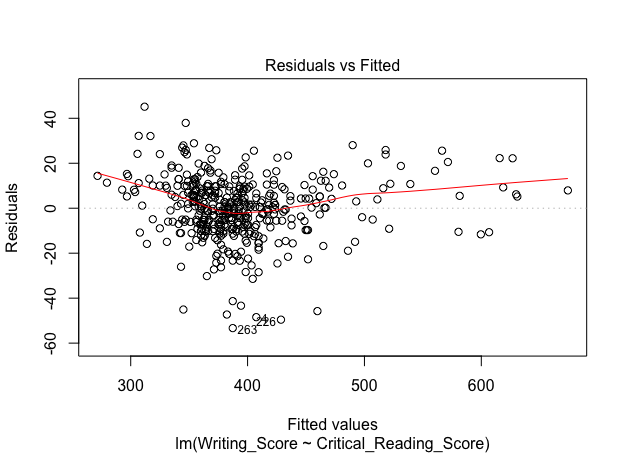
\includegraphics[scale=0.5]{both_removed_plots/fitted_vs_residual_altered_final}
%	\centering
%\end{figure}

We note that the confidence interval is narrower than in previous iterations, mostly due to the removal of two of the dataset's outliers. The Q-Q plot is much closer to showing an ideal distribution, with a slightly persistant left skew. Lastly, our plot  of fitted values with regards to residuals is getting closer and closer to having the slope center around 0. Our dataset contained a reasonable number of observations, although due to our particular analysis of the data -- our decision to base our writing score model around our critical reading score -- there aren't too many more paths to follow with regards to analyzing this dataset. 


\section*{Summary}
There seems to be a strong case in support of my assertion that the \textit{College Board} unfairly weighs the humanities on the SAT. Despite removing two outstanding outliers, our final regression model is incredibly close to our ideal model. With regards to our real-world problem, we can safely say that the SAT should restructure their exam in order to ensure an equal weighing of sections with respect to the other sections. \par
Understanding the weaknesses of a nationally-recognized standardized exam is vital to test-takers, educators, and the broader educational community. Should the \textit{College Board} consider redesigning their SAT exam, it would be sensible to consider adopting a subject structure that is more varied -- like the ACT's, whose four test sections (Science, Mathematics, English, Reading) not only span a wider variety of topics, but are also committed to evaluating a student equally between the more numerical/analytical and creative/humanties sections. \par
Despite our model's relative simplicity, I do feel that a simple linear regression model that utilizes critical reading score is more representative of an SAT test taker's performance on the writing section than a more involved, complex linear regression model that includes the mathematics section and other auxiliary features. Ideally, our results would have been more transparent if the dataset did not contain the averaged score of all college-bound seniors per observation -- rather, if each row contained a college-bound senior's scores, I strongly believe our data would have avoided any influences stemming from the mean. Furthermore, it would have been more ideal if our dataset had scores distributed across the past few years in order to be sure that the 2012 SAT exam was not just an anomaly within the history of SAT exams but that also would have proven much more difficult for a simple linear regression. \par
From this analysis, I've learned both peripheral skills and more directly-applied skills. Peripherally, the data collection and exploration phases of the analysis were useful in building data extraction and interpretation skills. While validating and cleaning my data in \textsc{R}, however, I gained more directly-applied skills with regards to programming, file I/O, and data visualization. During the data analysis and statistical reporting phase, there were instances where I was unsure as to how I should have approached this problem and, on numerous occassions, I considered restarting my analysis with a modified regression model or different dataset altogether. Ultimately, I learned more about statistical reporting and the data modeling/analysis process (going from question $\rightarrow$ data $\rightarrow$ model $\rightarrow$ analysis $\rightarrow$ results).

%----------------------------------------------------------------------------------------
% Resources
%----------------------------------------------------------------------------------------
\subsection*{Resources}
All files pertaining to this statistical report, including the \texttt{R} data analysis script, dataset, plots, and this PDF write-up are open to the public and hosted on GitHub (\href{https://github.com/dannyfig/MultivaRiate/tree/master/Problem_Set_1/}{\url{github.com/dannyfig/multivariate/problem_set_1}}).

%----------------------------------------------------------------------------------------
% Data
%----------------------------------------------------------------------------------------

\subsection*{Data}
Below is a slice (\textbf{pivoted in order to fit}) of the billboard dataset I utilized for this statistical analysis report. A few points to note are as follow:
\begin{enumerate}
	\item Originally, the parsed dataset provided 10 relevant features. Notably: \textbf{last week} (song's position last week, if applicable), \textbf{peak} (song's billboard peak), \textbf{weeks on chart}, \textbf{title}, \textbf{artist}, \textbf{chart entry date}, \textbf{entry position}, \textbf{overall weeks on chart}, \textbf{chart date} (date that data was recorded in YYYYMMDD format).
	\item Through some engineering within my \texttt{regression\_analysis.R} script, I was able to add a few more columns, including: \textbf{artist appearances} (how many times an artist was on the billboard for that recorded entry), FILL THIS IN
\end{enumerate}

\begin{table}[H]
	\centering
	\begin{tabular}{|l|c|c|}
		COLUMNS & row\_1 & row\_2 \\
		last week              & 1 & 2 \\
		peak                   & 1 & 2 \\
		weeks on chart         & 15 & 20 \\
		title                  & ``Uptown Funk!'' & ``Thinking out loud'' \\
		artist                 & ``MARK RONSON featuring BRUNO MARS'' & ``ED SHEERAN'' \\
		chart entry date       & 41972 & 41937 \\
		entry position         & 65 & 69 \\
		overall peak           & 1 & 2 \\
		overall weeks on chart & 15 & 20 \\
		chart date             & 20150307 & 20150307 \\
		artist appearances     & FILL THIS IN & FILL THIS IN\\
	\end{tabular}
\end{table}

%----------------------------------------------------------------------------------------

\end{document}